\chapter{Các định luật bất biến, bốn-vectơ và tenxơ trường}

Chúng ta sẽ bắt đầu bằng một định luật mà tự nhiên lẽ ra có thể tuân theo nhưng lại không tuân theo. Việc nó thất bại sẽ cho ta biết một định luật vật lý nên được viết như thế nào. Cùng phép kiểm tra ấy trước hết dẫn ta từ các thành phần tọa độ tới các vectơ thông thường, rồi từ các vectơ thông thường tới các bốn-vectơ, và cuối cùng từ các bốn-vectơ tới các tenxơ. Đến cuối cùng, điện trường và từ trường sẽ không còn là những đối tượng tách biệt: cùng nhau, chúng sẽ chiếm sáu vị trí độc lập của một tenxơ phản đối xứng.

Trừ khi có nói khác đi, chúng ta dùng hệ đơn vị trong đó \(c=1\), sắp thứ tự các thành phần không-thời gian là \((1,2,3,0)=(x,y,z,t)\), và dùng chữ ký metric \((-,-,-,+)\).

\section{Một định luật khả dĩ nhưng có đối xứng sai}

Hãy cố định một trục \(x\) và một trục \(y\) trong không gian. Bây giờ hãy quy định rằng hai hạt tương tác bất cứ khi nào các tọa độ \(x\) của chúng trùng nhau. Tương tác có thể đảo ngược chuyển động của chúng hoặc làm chúng đi ra theo những hướng mới; động lực học chi tiết của nó không quan trọng. Điều kiện kích hoạt được đề xuất đơn giản là
\begin{equation}
  x_1-x_2=0,
\end{equation}
trong đó các chỉ số dưới dùng để gắn nhãn các hạt chứ không phải các thành phần tọa độ. Không có mâu thuẫn toán học nào trong quy tắc này. Câu hỏi là điều gì khiến nó trở nên không hợp lý về mặt vật lý.

\begin{classroomqa}
\audiencequestion{Quy tắc này có vi phạm tính đồng nhất của không gian không?}
\lecturerresponse{Không. Tịnh tiến gốc tọa độ làm thay đổi cả hai tọa độ cùng một lượng và giữ \(x_1-x_2\) không đổi. Quy tắc này không chỉ ra vị trí ưu tiên nào. Khiếm khuyết của nó là tính đẳng hướng: nó chọn ra một phương ưu tiên.}
\end{classroomqa}

Hãy quay các trục đi \(90^\circ\). Phương \(x\) cũ nay được gọi là \(y\), vì thế cùng các sự kiện vật lý ấy sẽ được mô tả bằng sự bằng nhau của các tọa độ \(y\). Với một góc tổng quát, điều kiện sẽ liên quan tới một tổ hợp tuyến tính của \(x\) và \(y\). Do đó dạng của định luật phụ thuộc vào việc cái bảng được đặt theo hướng nào. Nó bất biến đối với tịnh tiến nhưng không bất biến đối với quay.

Chúng ta thường viết các định luật vật lý ở dạng đơn giản nhất trong các tọa độ trực giao. Có thể dùng các tọa độ tổng quát hơn, nhưng khi đó metric và các công thức trở nên kém đơn giản hơn. Trong lớp các hệ Descartes trực giao, không định hướng nào nên được ưu tiên.

Cách sửa là tức thì. Trong hai chiều, yêu cầu cả hai tọa độ phải trùng nhau; trong ba chiều, yêu cầu cả ba:
\begin{equation}
  x_1=x_2,
  \qquad y_1=y_2,
  \qquad z_1=z_2.
\end{equation}
Khi đó các hạt chỉ có thể tương tác khi chúng đến cùng một điểm, ngay cả nếu chúng tiến tới điểm ấy dọc theo các đường khác nhau.

\begin{classroomqa}
\audiencequestion{Các tọa độ \(z\) và thời gian có cũng phải trùng nhau không?}
\lecturerresponse{Trong không gian ba chiều, các tọa độ \(z\) cũng phải trùng nhau. Hiện thời gian đang được tạm gác sang một bên; nó sẽ được đưa trở lại ngay khi lập luận không gian hoàn tất.}
\end{classroomqa}

Gọi \(\boldsymbol r_a\) là vị trí của hạt \(a\). Ba điều kiện theo thành phần trở thành một phương trình vectơ,
\begin{equation}
  \boldsymbol r_1-\boldsymbol r_2=\boldsymbol 0.
\end{equation}
Một thành phần có thể triệt tiêu trong một hệ đã quay này và không triệt tiêu trong một hệ quay khác. Toàn bộ vectơ thì khác: nếu mọi thành phần đều bằng không trong một hệ, thì mọi thành phần đều bằng không trong mọi hệ quay. Tương tự, nếu hai vectơ bằng nhau trong một hệ, thì chúng vẫn bằng nhau sau khi cả hai được biến đổi.

\begin{figure}[H]
\centering
\includegraphics[width=0.78\textwidth]{lecture_06_figure_01.png}
\caption{Ba đẳng thức tọa độ khiến va chạm có nghĩa là trùng nhau trong không gian thay vì trùng nhau dọc theo một trục ưu tiên.}
\lectureframe{00:09:00}
\end{figure}

Đó là lý do vì sao các phương trình vectơ hữu ích. Các thành phần của chúng thay đổi, nhưng đối tượng ấy biến đổi một cách nhất quán. Một định luật được viết cho toàn bộ đối tượng có thể giữ nguyên dạng khi các tọa độ bị quay.

\section{Sự trùng nhau trong không-thời gian}

Bây giờ hãy thay trục không gian thẳng đứng bằng thời gian. Một quy tắc Newton có thể nói rằng hai sự thay đổi chuyển động chỉ xảy ra tại những thời điểm bằng nhau. Trong cơ học Newton, tính đồng thời được mọi quan sát viên quán tính chia sẻ, nên một quy tắc như vậy là khả dĩ. Trong thuyết tương đối hẹp, nó chọn ra một hệ quy chiếu ưu tiên. Các sự kiện đồng thời trong một hệ chưa chắc đồng thời trong một hệ khác.

Chỉ đòi hỏi các tọa độ không gian bằng nhau cũng không khá hơn. Một độ dời không-thời gian có thể có các thành phần không gian bằng không và một thành phần thời gian khác không,
\begin{equation}
  \Delta X^\mu=(0,0,0,\Delta t),
\end{equation}
và một phép boost trộn \(\Delta t\) với một thành phần không gian. Phát biểu địa phương bất biến là hai sự thay đổi chuyển động xảy ra tại cùng một sự kiện. Vì thế một va chạm đơn giản đòi hỏi
\begin{equation}
  X_1^\mu=X_2^\mu,
  \qquad\text{or}\qquad
  X_1^\mu-X_2^\mu=0.
\end{equation}
Cả bốn tọa độ đều trùng nhau: các hạt chiếm cùng một vị trí vào cùng một thời điểm.

Ví dụ va chạm cho ta một quy tắc tổng quát để viết vật lý. Ta có thể chuyển mọi thứ sang một vế và đặt một bốn-vectơ đầy đủ bằng không, hoặc đặt một bốn-vectơ đầy đủ bằng một bốn-vectơ đầy đủ khác. Chỉ riêng việc cho các mảnh rời rạc của một bốn-vectơ bằng nhau thì không tạo nên một phát biểu bất biến Lorentz.

\section{Các phép boost, phép quay và ký pháp ma trận}

Một bốn-vectơ là một đối tượng biến đổi theo cùng cách như một độ dời không-thời gian biến đổi. Để định nghĩa đó trở nên hữu ích, trước hết hãy nhắc lại các phép biến đổi của chính các tọa độ. Với một phép boost có tốc độ \(v\) theo hướng \(x\),
\begin{align}
  x'&=\gamma(x-vt), & y'&=y, & z'&=z,
  & t'&=\gamma(t-vx),                                      \label{eq:l6-boost}
\end{align}
trong đó
\begin{equation}
  \gamma(v)=\frac{1}{\sqrt{1-v^2}}.
\end{equation}

\begin{classroomqa}
\audiencequestion{Trong các công thức này có phải tốc độ ánh sáng đã được đặt bằng một không?}
\lecturerresponse{Đúng. Khi khôi phục đơn vị, hãy lấy \(X^0=ct\), thay \(1-v^2\) bằng \(1-v^2/c^2\), và khôi phục các thừa số \(c\) tương ứng trong các hạng hỗn hợp không gian--thời gian.}
\end{classroomqa}

Một phép quay quanh trục \(z\) trộn \(x\) và \(y\), để \(z\) và \(t\) đứng yên:
\begin{equation}
\begin{pmatrix}
  x'\\ y'\\ z'\\ t'
\end{pmatrix}
=
\begin{pmatrix}
  \cos\theta & \sin\theta & 0 & 0\\
  -\sin\theta & \cos\theta & 0 & 0\\
  0 & 0 & 1 & 0\\
  0 & 0 & 0 & 1
\end{pmatrix}
\begin{pmatrix}
  x\\ y\\ z\\ t
\end{pmatrix}.
\end{equation}
Các số 0 đáng được viết ra: chúng cho thấy tường minh thành phần nào không đi vào một tọa độ đã biến đổi cho trước. Với cùng thứ tự đó, phép boost trong phương trình~\eqref{eq:l6-boost} là
\begin{equation}
\begin{pmatrix}
  x'\\ y'\\ z'\\ t'
\end{pmatrix}
=
\begin{pmatrix}
  \gamma & 0 & 0 & -\gamma v\\
  0 & 1 & 0 & 0\\
  0 & 0 & 1 & 0\\
  -\gamma v & 0 & 0 & \gamma
\end{pmatrix}
\begin{pmatrix}
  x\\ y\\ z\\ t
\end{pmatrix}.
\end{equation}

Các phép quay và các phép boost có thể được hợp thành bằng phép nhân ma trận. Để boost theo một hướng không thẳng hàng với trục \(x\) ban đầu, ta có thể quay hướng ấy vào trục \(x\), áp dụng phép boost, rồi quay tiếp nếu cần. Các tích của những ma trận sơ cấp này sinh ra các phép biến đổi Lorentz tổng quát hơn.

\begin{classroomqa}
\audiencequestion{Việc quay trước rồi boost sau, hay boost trước rồi quay sau, có quan trọng không?}
\lecturerresponse{Có. Sau phép toán thứ nhất, các trục mà phép toán thứ hai tác dụng lên đã thay đổi. Hai tích ma trận không nhất thiết trùng nhau, nên thứ tự các phép toán là quan trọng.}
\end{classroomqa}

Tất cả các phép biến đổi tuyến tính này đều có thể được viết gộp lại thành
\begin{equation}
  X'^{\mu}=\Lambda^{\mu}{}_{\nu}X^{\nu}.                  \label{eq:l6-vector-transform}
\end{equation}
Chỉ số lặp \(\nu\) được lấy tổng trên \(1,2,3,0\). Đây đơn giản là tổng hàng nhân cột quen thuộc trong phép nhân ma trận, được biểu diễn bằng ký pháp chỉ số.

\begin{figure}[H]
\centering
\includegraphics[width=0.78\textwidth]{lecture_06_figure_02.png}
\caption{Phép biến đổi Lorentz viết theo chỉ số, ở phía trên phần mở đầu của dạng vectơ cột của nó.}
\lectureframe{00:31:55}
\end{figure}

Phương trình~\eqref{eq:l6-vector-transform} cũng là định nghĩa của một bốn-vectơ phản biến tổng quát. Nếu \(A^\mu\) là một vectơ như vậy, thì
\begin{equation}
  A'^{\mu}=\Lambda^{\mu}{}_{\nu}A^{\nu}.
\end{equation}
Bốn thành phần của nó không nhất thiết biểu diễn vị trí. Điều làm cho đối tượng ấy là một bốn-vectơ chính là quy luật biến đổi của nó.

\section{Vô hướng, metric và các tích bất biến}

Trước khi dùng thêm các bốn-vectơ, sẽ hữu ích nếu lùi lại khái niệm đơn giản hơn là đại lượng vô hướng. Dưới các phép quay trong không gian, nhiệt độ tại một điểm xác định là một vô hướng, và khoảng cách giữa hai điểm xác định cũng vậy. Mỗi cái là một con số, không phụ thuộc vào định hướng của các trục. Thậm chí người ta còn có thể đưa ra một khẳng định số học cố ý ngớ ngẩn rằng một khoảng cách đo bằng xentimét bằng nhiệt độ căn phòng đo bằng độ Fahrenheit. Khẳng định ấy không có chiều sâu vật lý, nhưng vì cả hai vế đều là các vô hướng dưới phép quay, tính đúng hay sai của nó không phụ thuộc vào việc các trục được quay thế nào.

Các thành phần của một vectơ không phải là các vô hướng. Vì vậy ta cần một cách có hệ thống để kết hợp chúng thành các vô hướng. Hãy viết một bốn-vectơ phản biến tổng quát là
\begin{equation}
  A^\mu=(A^1,A^2,A^3,A^0).
\end{equation}
Các thành phần hiệp biến mô tả cùng một đối tượng hình học nhưng với chỉ số ở dưới. Với chữ ký của ta, chúng thu được bằng cách dùng metric Minkowski,
\begin{equation}
  A_\mu=\eta_{\mu\nu}A^\nu,
  \qquad
  \eta_{\mu\nu}=
  \begin{pmatrix}
    -1&0&0&0\\
    0&-1&0&0\\
    0&0&-1&0\\
    0&0&0&1
  \end{pmatrix},                                          \label{eq:l6-metric}
\end{equation}
để rồi
\begin{equation}
  A_\mu=(-A^1,-A^2,-A^3,A^0).
\end{equation}

\begin{classroomqa}
\audiencequestion{Hai chỉ số và các dấu trên bảng có mâu thuẫn với nhau không?}
\lecturerresponse{Có. Thành phần không gian trong cột được hiển thị cần dấu trừ tương ứng, và các thành phần ở vế phải của phương trình hạ chỉ số mang chỉ số trên trước khi nhân với \(\eta_{\mu\nu}\). Nhãn thời gian là \(0\), không phải \(4\).}
\end{classroomqa}

\begin{figure}[H]
\centering
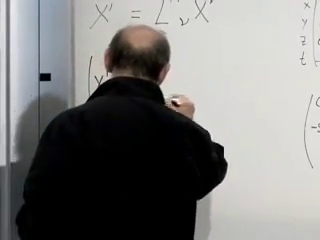
\includegraphics[width=0.8\textwidth]{lecture_06_figure_03.png}
\caption{Các thành phần phản biến và hiệp biến, ma trận metric, và phần mở đầu của phép co bất biến.}
\lectureframe{00:45:00}
\end{figure}

Hạ chỉ số không phải là trang trí. Nó gói gọn các dấu cần thiết cho chuẩn bất biến Lorentz:
\begin{align}
  A_\mu A^\mu
  &=-(A^1)^2-(A^2)^2-(A^3)^2+(A^0)^2,                    \label{eq:l6-norm}\\
  X_\mu X^\mu
  &=t^2-x^2-y^2-z^2.
\end{align}
Biểu thức thứ hai là khoảng không-thời gian bất biến tính từ gốc. Vì \(A^\mu\) biến đổi theo cùng cách như \(X^\mu\), phép co của nó cũng có cùng tính bất biến.

Ký pháp ấy cũng dạy một quy tắc ghi chép hữu ích. Một chỉ số lấy tổng lặp lại xuất hiện một lần ở trên và một lần ở dưới. Ví dụ,
\begin{equation}
  A_\mu A^\mu
  =\eta_{\mu\nu}A^\mu A^\nu.
\end{equation}
Tên của các chỉ số được lấy tổng, hay chỉ số giả, có thể thay đổi mà không làm thay đổi đại lượng.

\begin{classroomqa}
\audiencequestion{Có nên xem một trong các vectơ này là một hàng và cái kia là một cột không, và thứ tự của chúng có quan trọng không?}
\lecturerresponse{Đối với phép tính hiện tại, hãy xem các đại lượng có chỉ số là các thành phần và để metric thực hiện phép co; không cần biến cuộc thảo luận thành đại số toán tử hàng-đối-cột. Đây là các số thông thường, nên thứ tự của chúng không quan trọng. Các toán tử không giao hoán sẽ đòi hỏi cẩn thận hơn, nhưng đó không phải là chủ đề ở đây.}
\end{classroomqa}

Cùng phép xây dựng ấy cho một tích trong giữa hai bốn-vectơ khác nhau,
\begin{equation}
  A\mathbin{\cdot}B=A_\mu B^\mu=A^\mu B_\mu.
\end{equation}
Tính bất biến của nó suy ra mà không cần viết ra một ma trận Lorentz tường minh. Vì \(A+B\) và \(A-B\) là các bốn-vectơ, nên cả hai chuẩn bình phương của chúng đều bất biến:
\begin{align}
  (A+B)^2&=A^2+B^2+2A\mathbin{\cdot}B,\\
  (A-B)^2&=A^2+B^2-2A\mathbin{\cdot}B.
\end{align}
Lấy hiệu cho ta
\begin{equation}
  (A+B)^2-(A-B)^2=4A\mathbin{\cdot}B,                    \label{eq:l6-polarization}
\end{equation}
vì thế \(A\mathbin{\cdot}B\) cũng bất biến. Hệ số 4 suy ra trực tiếp từ phép khai triển.\editorialnote{Lập luận trên bảng cung cấp đồng nhất thức phân cực này; việc viết ra hệ số ấy làm cho phép triệt tiêu được nói bằng lời trở nên không mơ hồ.}

\begin{figure}[H]
\centering
\includegraphics[width=0.8\textwidth]{lecture_06_figure_04.png}
\caption{Hai bình phương bất biến được dùng để tách ra tích trong của hai bốn-vectơ khác nhau.}
\lectureframe{00:52:20}
\end{figure}

Các đại lượng bất biến là những thành phần tự nhiên của các định luật vật lý: khác với một thành phần riêng lẻ, chúng mang cùng một giá trị từ hệ quy chiếu này sang hệ quy chiếu khác.

\section{Vận tốc riêng và bốn-động lượng}

Xét hai sự kiện lân cận trên đường thế giới của một hạt. Độ tách của chúng là vi phân bốn-vectơ
\begin{equation}
  dX^\mu=(dx,dy,dz,dt).
\end{equation}
Với một đường thế giới loại thời, thời gian riêng được định nghĩa bởi
\begin{equation}
  d\tau^2=dX_\mu dX^\mu
  =dt^2-dx^2-dy^2-dz^2.                                  \label{eq:l6-proper-time}
\end{equation}
Bốn-vận tốc riêng là
\begin{equation}
  U^\mu=\frac{dX^\mu}{d\tau}.                            \label{eq:l6-four-velocity}
\end{equation}
Nó đo tốc độ biến thiên của vị trí không-thời gian theo thời gian riêng của chính hạt, chứ không theo thời gian tọa độ của một hệ quy chiếu được chọn.

Mặc dù \(U^\mu\) có bốn thành phần, chỉ có ba trong số đó là độc lập. Chia phương trình~\eqref{eq:l6-proper-time} cho \(d\tau^2\) ta được
\begin{equation}
  U_\mu U^\mu=1.
\end{equation}
Do đó bốn-vận tốc là một vectơ loại thời đơn vị. Việc chọn hướng về tương lai cố định dấu của thành phần thời gian của nó.

\begin{classroomqa}
\audiencequestion{Ở các tốc độ nhỏ hơn rất nhiều so với \(c\), bốn-vận tốc có suy biến thành vận tốc thông thường không?}
\lecturerresponse{Ba thành phần không gian của nó tiến tới vận tốc thông thường, còn thành phần thời gian của nó tiến tới một theo đơn vị \(c=1\). Hệ thức ấy suy ra bằng cách áp dụng quy tắc chuỗi và tính \(dt/d\tau\).}
\end{classroomqa}

Đối với mỗi thành phần không gian,
\begin{equation}
  U^i=\frac{dx^i}{d\tau}
     =\frac{dx^i}{dt}\frac{dt}{d\tau}
     =v^i\frac{dt}{d\tau}.
\end{equation}
Hãy chia phương trình~\eqref{eq:l6-proper-time} cho \(dt^2\):
\begin{equation}
  \left(\frac{d\tau}{dt}\right)^2
  =1-v_x^2-v_y^2-v_z^2
  =1-\boldsymbol v^2.
\end{equation}
Vì thế
\begin{equation}
  \frac{dt}{d\tau}=\frac{1}{\sqrt{1-\boldsymbol v^2}}
  =\gamma(\lvert\boldsymbol v\rvert),
\end{equation}
và
\begin{equation}
  U^\mu=(\gamma v_x,\gamma v_y,\gamma v_z,\gamma).
                                                                  \label{eq:l6-u-components}
\end{equation}

\begin{figure}[H]
\centering
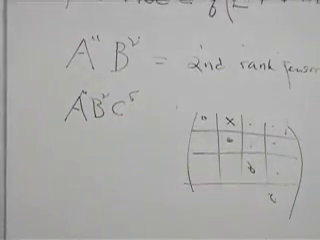
\includegraphics[width=0.8\textwidth]{lecture_06_figure_05.png}
\caption{Phép tính thời gian riêng cho ra \(dt/d\tau=\gamma\) và liên hệ vận tốc riêng với vận tốc thông thường.}
\lectureframe{01:02:00}
\end{figure}

\begin{classroomqa}
\audiencequestion{Liệu \(dx^2/dt^2\) có nghĩa là đạo hàm bậc hai không, và việc bình phương một vectơ có nên sinh ra các hạng chéo không?}
\lecturerresponse{Ở đây nó có nghĩa là \((dx/dt)^2\), tức bình phương của một đạo hàm bậc nhất. Hơn nữa, \(\boldsymbol v^2\) có nghĩa là tích vô hướng Euclid \(v_x^2+v_y^2+v_z^2\), chứ không phải bình phương của tổng hình thức \(v_x+v_y+v_z\); không có các hạng chéo.}
\end{classroomqa}

\begin{classroomqa}
\audiencequestion{Trong \(\gamma(v)\), \(v\) là tốc độ tương đối giữa hai hệ quy chiếu hay là tốc độ của hạt?}
\lecturerresponse{Ở đây, đó là tốc độ của hạt trong hệ quy chiếu đã chọn. Hàm \(\gamma(v)=1/\sqrt{1-v^2}\) có thể được tính cho bất kỳ tốc độ nào: trong một phép biến đổi boost, nó được tính tại tốc độ tương đối của các hệ quy chiếu; còn trong bốn-vận tốc, nó được tính tại tốc độ của hạt.}
\end{classroomqa}

Với \(v\ll1\), \(\gamma\simeq1\), nên các thành phần không gian của \(U^\mu\) tiến tới \(\boldsymbol v\) và \(U^0\) tiến tới một. Khi tốc độ thông thường tiến gần tới tốc độ ánh sáng, \(\gamma\) và mọi thành phần khác không của bốn-vận tốc đều tăng vô hạn.

\begin{classroomqa}
\audiencequestion{Không phải \(U^0\) nên có đơn vị của vận tốc thay vì gần bằng số 1 sao?}
\lecturerresponse{Các đơn vị biến mất khi đặt \(c\) bằng 1. Với \(X^0=ct\), ta có
\(U^\mu=(\gamma\boldsymbol v,\gamma c)\), nên thành phần thời gian tiến tới
\(c\) và \(U_\mu U^\mu=c^2\).}
\end{classroomqa}

Đối với một hạt có khối lượng nghỉ \(m\), định nghĩa bốn-động lượng bởi
\begin{equation}
  P^\mu=mU^\mu.
\end{equation}
Trong đơn vị tự nhiên,
\begin{equation}
  P^\mu=(\gamma m\boldsymbol v,\gamma m).
\end{equation}
Ba thành phần đầu tiên tiến tới động lượng Newton \(m\boldsymbol v\) ở tốc độ thấp. Khôi phục đơn vị, ta được
\begin{equation}
  P^\mu=(\gamma m\boldsymbol v,E/c),
  \qquad E=\gamma mc^2,
\end{equation}
và do đó
\begin{equation}
  E=mc^2+\frac{1}{2}m\boldsymbol v^2+O(mv^4/c^2).
\end{equation}
Thành phần thời gian là năng lượng trong đơn vị \(c=1\), hoặc là năng lượng chia cho \(c\) khi cả bốn thành phần đều được gán đơn vị động lượng.

\begin{classroomqa}
\audiencequestion{Liệu \(\boldsymbol v\) thông thường, với một thành phần thứ tư được thêm vào, tự nó có phải là một bốn-véc-tơ không?}
\lecturerresponse{Không. Ba-vận tốc thông thường không biến đổi như một bốn-véc-tơ. Thừa số \(\gamma\) và định nghĩa theo thời gian riêng là thiết yếu; bốn-véc-tơ là \(U^\mu\), không phải \(\boldsymbol v\).}
\end{classroomqa}

\section{Vì sao điện trường và từ trường phải trộn lẫn}

Bây giờ ta tạm nghỉ ngắn khỏi thuyết tương đối, như vừa nói. Hãy bắt đầu với phương trình chuyển động trước Einstein và hỏi xem nó phải được tổ chức lại như thế nào thì mới có thể đúng trong mọi hệ quán tính. Gia tốc thông thường là đạo hàm theo thời gian của vận tốc thông thường. Tương tự bốn chiều của nó một cách tự nhiên là
\begin{equation}
  A^\mu=\frac{dU^\mu}{d\tau}.
\end{equation}
Ở tốc độ thấp, các thành phần không gian của nó tiến tới gia tốc thông thường. Phương trình tương đối tính đầy đủ sẽ được để lại sau; trước hết hãy xét luật lực cũ.

Đối với một điện tích \(q\) trong điện trường và từ trường,
\begin{equation}
  \boldsymbol F=m\boldsymbol a
  =q\left(\boldsymbol E+\boldsymbol v\times\boldsymbol B\right).
                                                                  \label{eq:l6-lorentz-force}
\end{equation}
Hạng điện không phụ thuộc vào vận tốc của hạt, còn hạng từ thì có phụ thuộc.

\begin{figure}[H]
\centering
\includegraphics[width=0.8\textwidth]{lecture_06_figure_06.png}
\caption{Dạng tiền tương đối tính của định luật lực Lorentz, gợi ý việc kết hợp \(\boldsymbol E\) và \(\boldsymbol B\).}
\lectureframe{01:18:20}
\end{figure}

Giả sử một quan sát viên không thấy điện trường nhưng lại thấy từ trường và một điện tích đang chuyển động. Điện tích ấy chịu một lực từ. Tuy nhiên, trong hệ quy chiếu nghỉ tức thời của điện tích, \(\boldsymbol v=0\), nên số hạng từ trong phương trình~\eqref{eq:l6-lorentz-force} triệt tiêu. Đường thế giới vật lý không trở thành quán tính chỉ vì tọa độ đã thay đổi; vì vậy lực trong hệ mới phải bao gồm một thành phần điện. Nói chính xác hơn, không thể biến đổi một bốn-gia tốc khác không thành bằng không chỉ bằng cách đổi hệ quy chiếu quán tính, mặc dù gia tốc ba chiều và các thành phần của nó quả thật có biến đổi. \editorialnote{Mệnh đề về bốn-gia tốc này là dạng bất biến của lập luận quen thuộc trên lớp học và tránh coi chính gia tốc ba chiều thông thường là bất biến theo hệ quy chiếu.}

Do đó, điện trường và từ trường phải biến đổi thành nhau. Gộp lại, chúng có 6 thành phần, nên chúng không phải là một vô hướng cũng không phải là một bốn-véc-tơ. Ta cần một đối tượng biến đổi mới.

\section{Tensor: mỗi chỉ số ứng với một phép biến đổi}

Một đại lượng vô hướng có thể được gọi là tensor hạng 0; nó không có chỉ số. Một bốn-véc-tơ là tensor hạng 1; nó có một chỉ số với 4 giá trị có thể có. Ví dụ đơn giản nhất về hạng 2 là tích
\begin{equation}
  A^\mu B^\nu.
\end{equation}
Mỗi chỉ số có 4 giá trị, nên đối tượng này có \(4^2=16\) thành phần, có thể được biểu diễn thành một mảng \(4\times4\). Tích của ba véc-tơ,
\begin{equation}
  A^\mu B^\nu C^\sigma,
\end{equation}
có \(4^3=64\) thành phần và là một tensor hạng 3. Các hạng cao hơn tiếp tục theo mẫu đó. Tên gọi kém quan trọng hơn quy tắc xác định đối tượng.

Nếu
\begin{equation}
  A'^{\mu}=\Lambda^\mu{}_{\nu}A^\nu,
  \qquad
  B'^{\sigma}=\Lambda^\sigma{}_{\tau}B^\tau,
\end{equation}
thì tích của chúng biến đổi theo
\begin{equation}
  A'^{\mu}B'^{\sigma}
  =\Lambda^\mu{}_{\nu}\Lambda^\sigma{}_{\tau}
   A^\nu B^\tau.
\end{equation}
Điều này cho ta định luật định nghĩa cho một tensor phản biến hạng 2:
\begin{equation}
  T'^{\mu\sigma}
  =\Lambda^\mu{}_{\nu}\Lambda^\sigma{}_{\tau}T^{\nu\tau}.
                                                                  \label{eq:l6-tensor-transform}
\end{equation}
Có một ma trận Lorentz cho mỗi chỉ số. Các chỉ số lặp \(\nu\) và \(\tau\) được lấy tổng; các chỉ số tự do \(\mu\) và \(\sigma\) ghi nhãn thành phần đang được tính trong hệ có dấu phẩy.

\begin{figure}[H]
\centering
\includegraphics[width=0.82\textwidth]{lecture_06_figure_07.png}
\caption{Phép biến đổi của hai véc-tơ và hệ quả là định luật biến đổi với hai ma trận cho một tensor hạng 2.}
\lectureframe{01:27:15}
\end{figure}

Một tensor không nhất thiết phải là một tích đơn lẻ của các véc-tơ. Cả \(A^\mu B^\nu\) và \(A^\nu B^\mu\) đều tuân theo định luật biến đổi tensor, cũng như tổng của chúng và mọi tổng như
\begin{equation}
  A^\mu B^\nu+C^\mu D^\nu.
\end{equation}
Chính định luật biến đổi, chứ không phải một cách phân tích thừa số cụ thể, mới là định nghĩa. Một tensor hạng 3 nhận thêm ma trận Lorentz thứ ba, và cứ thế tiếp tục.

\section{Tensor đối xứng và phản đối xứng}

Hai lớp tensor hạng 2 sẽ đặc biệt hữu ích. Một tensor đối xứng thỏa mãn
\begin{equation}
  T^{\mu\nu}=T^{\nu\mu},
\end{equation}
nên các phần tử đối xứng qua đường chéo là như nhau. 4 phần tử trên đường chéo và 6 phần tử ở một phía của đường chéo xác định phần còn lại, cho
\begin{equation}
  4+6=10
\end{equation}
thành phần độc lập.

Một tensor phản đối xứng thỏa mãn
\begin{equation}
  T^{\mu\nu}=-T^{\nu\mu}.                                \label{eq:l6-antisymmetry}
\end{equation}
Thay \(\mu=\nu\) vào phương trình~\eqref{eq:l6-antisymmetry} thì được
\(T^{\mu\mu}=-T^{\mu\mu}\), nên mọi phần tử trên đường chéo đều triệt tiêu. 6 phần tử trong một nửa tam giác xác định 6 phần tử kia qua đổi dấu. Vì vậy có đúng 6 thành phần độc lập.

\begin{figure}[H]
\centering
\includegraphics[width=0.82\textwidth]{lecture_06_figure_08.png}
\caption{Một mảng \(4\times4\) phản đối xứng hoàn chỉnh: các số 0 trên đường chéo và các dấu đối nhau qua nó.}
\lectureframe{01:34:25}
\end{figure}

Chính cách đếm đó là đầu mối. 3 thành phần điện và 3 thành phần từ có thể đặt gọn trong một tensor phản đối xứng hạng 2.

\section{Tensor trường điện từ}

Hãy cho các nhãn không-thời gian chạy theo các hàng và cột theo thứ tự
\((1,2,3,0)=(x,y,z,t)\). Cách sắp xếp được viết trên bảng là
\begin{equation}
  F_{\mu\nu}=
  \begin{pmatrix}
    0    & -B_3 & B_2  & E_1\\
    B_3  & 0    & -B_1 & E_2\\
    -B_2 & B_1  & 0    & E_3\\
    -E_1 & -E_2 & -E_3 & 0
  \end{pmatrix}.                                         \label{eq:l6-field-tensor}
\end{equation}
Các ô thuần không gian chứa từ trường; các ô mang một chỉ số không gian và một chỉ số thời gian chứa điện trường. Tính phản đối xứng cho các phần tử tam giác dưới một khi đã biết các phần tử tam giác trên.

\begin{classroomqa}
\audiencequestion{Các phần tử từ có phải đều âm không, và các nhãn có tương ứng với \(x,y,z\) không?}
\lecturerresponse{Các dấu trong tam giác không gian phía trên luân phiên như đã chỉ ra:
\(-B_3,+B_2,-B_1\). Các nhãn \(1,2,3\) tương ứng với \(x,y,z\), còn
\(0\) gắn với thời gian. Phản xạ qua đường chéo đảo mọi dấu.}
\end{classroomqa}

\begin{figure}[H]
\centering
\includegraphics[width=0.82\textwidth]{lecture_06_figure_09.png}
\caption{Tensor trường điện từ hoàn chỉnh theo thứ tự thành phần lấy không gian trước của bài giảng.}
\lectureframe{01:41:05}
\end{figure}

Ký hiệu theo quy ước là \(F_{\mu\nu}\), chứ không phải một \(T_{\mu\nu}\) tổng quát. Giảng viên phỏng đoán rằng chữ cái ấy có thể ám chỉ Faraday, đồng thời nói rõ rằng ông không biết lịch sử của ký hiệu đó. Điều quan trọng ở đây là tính phản đối xứng của nó và 6 thành phần trường của nó, chứ không phải phỏng đoán ấy về chữ cái.

\begin{classroomqa}
\audiencequestion{Mỗi phần tử của ma trận có biểu diễn độ mạnh của một trường trong mặt phẳng tọa độ được chỉ ra không?}
\lecturerresponse{Đó là một thành phần của tensor trường điện từ. Các phần tử liên quan đến thời gian là các thành phần điện, còn các phần tử không gian--không gian mã hóa các thành phần từ.}
\end{classroomqa}

Hãy tách riêng hàng và cột mang chỉ số thời gian. Khối phản đối xứng \(3\times3\) còn lại là phần từ. Có thể nhớ các phần tử độc lập của nó theo chu kỳ:
\begin{equation}
  F_{12}=-B_3,
  \qquad F_{23}=-B_1,
  \qquad F_{31}=-B_2.                                   \label{eq:l6-magnetic-cycle}
\end{equation}
Bắt đầu từ hệ thức đầu tiên, dịch mọi nhãn theo vòng
\(1\to2\to3\to1\). Tương đương,
\begin{equation}
  F_{ij}=-\epsilon_{ijk}B_k,
\end{equation}
với \(\epsilon_{123}=+1\).\editorialnote{Công thức Levi--Civita là dạng chuẩn gọn của quy tắc tuần hoàn đã được triển khai tường minh trên bảng.}

\begin{figure}[H]
\centering
\includegraphics[width=0.82\textwidth]{lecture_06_figure_10.png}
\caption{Các thành phần không gian theo chu kỳ mã hóa từ trường trong tensor phản đối xứng.}
\lectureframe{01:46:20}
\end{figure}

Việc nhận dạng các thành phần điện thì trực tiếp hơn:
\begin{equation}
  E_1=F_{10},
  \qquad E_2=F_{20},
  \qquad E_3=F_{30}.
\end{equation}

Do đó, từ trường có hai cách đồng nhất hữu ích. Trong không gian ba chiều, một véc-tơ trục ba thành phần có thể được ghép cặp với một tensor phản đối xứng \(3\times3\). Tuy nhiên, trong không-thời gian, nó chỉ là phần không gian của tensor 6 thành phần \(F_{\mu\nu}\). Sự ghép cặp này là đặc biệt cho 3 chiều: một tensor phản đối xứng \(4\times4\) có 6 thành phần độc lập và không thể được đồng nhất với một bốn-véc-tơ.
\editorialnote{Dưới các phép quay đúng, từ trường ứng xử như một véc-tơ; dưới các phép phản xạ, chính xác hơn nó là một véc-tơ trục, hay giả véc-tơ.}

Mục đích của phép xây dựng này không phải là đếm thành phần chỉ vì bản thân việc đó. Vì \(F_{\mu\nu}\) biến đổi như một tensor, một phép boost Lorentz tự động trộn các phần tử điện và từ của nó. Trong bài giảng tiếp theo, nó có thể được kết hợp với bốn-vận tốc và bốn-gia tốc để thay phương trình~\eqref{eq:l6-lorentz-force} bằng một phương trình chuyển động hiệp biến.

\section{Các câu hỏi về Einstein và Minkowski}

Những phút cuối chuyển từ phần hình thức sang cách nó nảy sinh trong lịch sử. Các câu trả lời được đưa ra như những hồi tưởng hơn là một lịch sử đã được xác lập, và chính sự bảo lưu đó là một phần của cuộc trao đổi.

\begin{classroomqa}
\audiencequestion{Einstein tìm kiếm một cách phát biểu bất biến Lorentz vì lý do khái niệm, hay ông bị thúc đẩy bởi những quan sát cụ thể?}
\lecturerresponse{Nguyên lý rằng các định luật tự nhiên phải có cùng dạng trong mọi hệ quán tính là trung tâm trong lập luận của ông. Cũng có bằng chứng thực nghiệm liên quan đến ánh sáng và sự thất bại trong việc phát hiện chuyển động qua một ête, mặc dù giảng viên nói rõ rằng ông không chắc Einstein biết những kết quả nào hoặc chúng ảnh hưởng đến ông mạnh đến mức nào. Sức ép về mặt khái niệm là các phương trình Maxwell và lực Lorentz phải tuân theo nguyên lý tương đối, điều này đòi hỏi điện trường, từ trường và các thành phần vận tốc phải cùng biến đổi.}
\end{classroomqa}

Trình bày năm 1905 của Einstein không dùng ký pháp bốn-véc-tơ gọn như ở đây. Nó làm việc theo từng thành phần, với các thừa số cần thiết của \(\gamma\) và vận tốc được viết tường minh. Sau đó Minkowski tổ chức cùng một cấu trúc ấy về mặt hình học như không-thời gian bốn chiều.

\begin{classroomqa}
\audiencequestion{Einstein có chống lại cách phát biểu không-thời gian của Minkowski không, và Minkowski đã đưa nó ra sớm đến mức nào?}
\lecturerresponse{Hồi ức được nêu trong lớp là Einstein ban đầu không đón nhận ngôn ngữ hình học bốn chiều nhưng nhanh chóng chấp nhận giá trị của nó. Mốc thời gian được nêu một cách dè dặt là vào khoảng 2 năm sau bài báo 1905, có lẽ là 1907; người nói nhấn mạnh rằng ông đang hồi tưởng chứ không phải xác lập lịch sử.}
\end{classroomqa}

\begin{classroomqa}
\audiencequestion{Minkowski là nhà toán học hay nhà vật lý, ông còn đóng góp gì khác, và ông có chịu ảnh hưởng của Lorentz hay FitzGerald không?}
\lecturerresponse{Không có câu trả lời chắc chắn nào được khẳng định. Sự phân biệt giữa nhà toán học và nhà vật lý không được theo đuổi đến cùng, một sự đính chính từ khán giả ngắt lời một nhận xét khái quát về công trình khác của Minkowski, và các tuyến ảnh hưởng khả dĩ được để ngỏ một cách minh nhiên. Điểm chắc chắn cho cuộc thảo luận này là vai trò quyết định của Minkowski trong việc tổ chức thuyết tương đối bằng ký pháp hình học bốn chiều.}
\end{classroomqa}

\begin{classroomqa}
\audiencequestion{Các phép biến đổi trộn \(\boldsymbol E\) và
\(\boldsymbol B\) đã có sẵn trong công trình 1905 của Einstein chưa?}
\lecturerresponse{Có, nhưng được viết theo từng thành phần chứ không phải như một phương trình tensor trường duy nhất. Sự so sánh được nêu trong lớp là với các phương trình thành phần của Maxwell: nội dung có thể đã hiện diện trước cả ký pháp gọn làm lộ ra cấu trúc chung của nó. Đóng góp của Minkowski là làm cho cấu trúc ấy trở nên có hệ thống trong ngôn ngữ không-thời gian.}
\end{classroomqa}

Điều đó đưa ta trở lại điểm toán học mà từ đó ta đã bắt đầu. Các thành phần là không thể thiếu cho việc tính toán, nhưng định luật trở nên sáng tỏ khi các thành phần ấy được nhận ra là những phần của một đối tượng duy nhất biến đổi. Nhiệm vụ tiếp theo là dùng \(F_{\mu\nu}\) để viết phương trình chuyển động của hạt mang điện dưới một dạng có cùng hình thức trong mọi hệ quy chiếu quán tính.
